
\newcommand{\nomedoc}{Piano di Progetto}
\newcommand{\versione}{0.2}
\newcommand{\versioneglossario}{1.0}
\newcommand{\versionenormeprogetto}{1.0}
\newcommand{\nomefile}{PianoDiProgetto-\versione.pdf}
\newcommand{\datacreazione}{11 Dicembre 2010}
\newcommand{\datamodifica}{13 Dicembre 2010}
\newcommand{\stato}{formale}
\newcommand{\uso}{esterno}
\newcommand{\redazione}{Mandolo Andrea\\&Lovato Daniele}
\newcommand{\verifica}{---}
\newcommand{\approvazione}{---}
\newcommand{\distribuzione}{
VT.G \\
& Prof. Vardanega Tullio\\
& Prof. Cardin Riccardo }

% FUNZIONI TIPOGRAFICHE
\newcommand{\co}{\texttt} % courier
\newcommand{\bo}{\textbf} % bold
\newcommand{\pr}{\par\medskip} % paragrafo spaziato
\newcommand{\sca}{\textsc} % small caps

\documentclass[a4paper,12pt]{report}
% 10pt,11pt,12pt
% titlepage, notitlepage -> per dare inizio o no ad una nuova pagina dopo titolo
% twoside -> per dire se fronte-retro
\usepackage[latin1]{inputenc}
% per caratteri accentati
\usepackage[italian]{babel}
% per regole sintattiche italiane
\usepackage[bookmarks=true, pdfborder={0 0 0 0}]{hyperref}
% per collegamenti ipertestuali
\usepackage{graphicx}
% per inserimento immagini

% \usepackage{enumerate}
% per personalizzare elenchi puntati

\usepackage[hmargin=2cm]{geometry} %margine 2 cm
%\geometry{options varie}

% comandi per gestire meglio header e footer
\usepackage{fancyhdr}  % header e footer
\usepackage{totpages}
\pagestyle{fancy}
\renewcommand{\headrulewidth}{0.4pt}
\renewcommand{\footrulewidth}{0.4pt}

\setlength{\headheight}{1.2cm} % NON TOCCARE
\setlength{\voffset}{-1.5cm} % NON TOCCARE
\setlength{\textheight}{666pt} % NON TOCCARE
\setlength{\footskip}{60pt}
\setlength{\parindent}{0pt} % INDENTAZIONE

\lhead{\nomedoc\  (ver. \versione)}
\chead{}
\rhead{
\includegraphics[height=1cm]{img/netmus.png}}
\lfoot{
\includegraphics[height=0.8cm]{img/logo.png}}
\cfoot{}
\rfoot{\thepage}

\usepackage{titlesec}
\titleformat{\chapter}{\normalfont\huge\bfseries}
{\thechapter}{20pt}{\Huge}

\usepackage{rotating}   % PER TABELLE E AMBIENTI RUOTATI
\usepackage{array}
\usepackage{color}
\usepackage{colortbl}  % VARIE PER GESTIRE I COLORI
\definecolor{Orange}{RGB}{255,127,0}   % ARANCIO ACCES0
\definecolor{orange}{RGB}{255,207,80}  % ARANCIO TENUE

\addtocontents{toc}{\protect\thispagestyle{fancy}}  % PER INDICI CON + PAGINE
\usepackage[font=it]{caption}    % PER RENDERE CORSIVE LE DIDASCALIE
\usepackage{eurosym}  % PER SIMBOLO EURO

% \usepackage{listings}   per codice sorgente

\author{VT.G - Valter Texas Group}

\usepackage[table]{xcolor}   % AGGIUNGERE
\usepackage{eurosym}

\begin{document}

\pagenumbering{Roman} % INIZIO NUMERAZIONE ARABA

\vspace*{1cm}
\begin{center}

\begin{LARGE} \sca{Federico Baron} \end{LARGE}\\
\vspace{0.5cm}
\begin{Large}
\emph{fede.baron.89@gmail.com} \end{Large}\\
\vspace*{1cm} 
\includegraphics[width=5cm]{img/logo.png}\\
\vspace{0.5cm}
\begin{Large} \emph{``Comunicazione Aumentata/Alternativa per Giovani Ospiti
della Terapia Intensiva Pediatrica''} \end{Large}\\
\vspace{3cm}
\begin{Large} \sca{\nomedoc} \end{Large}\\
\end{center}
\vspace{1cm}

% INFORMAZIONI DOCUMENTO
\begin{center}
\begin{tabular}{r|l}
\hline & \\
\bo{Nome} & \nomefile \\
\bo{Versione attuale} & \versione \\
\bo{Data creazione} & \datacreazione \\
\bo{Data ultima modifica} & \datamodifica \\
\bo{Redazione} & \redazione \\
& \\\hline
\end{tabular}
\end{center}
\newpage

% REGISTRO MODIFICHE
\section*{Registro delle modifiche}
\begin{tabular}{lll}
% REVISIONI DEL DOCUMENTO
% DALLA PIU' NUOVA ALLA PIU' VECCHIA

\bo{Data:} 13/12/2010 &
\bo{Versione:} 0.2 &
\bo{Autore:} Mandolo Andrea\\
\hline\\
\multicolumn{3}{p{470px}}{ Completati contenuti dei capitoli 2-3-4.}\\ \\

\bo{Data:} 11/12/2010 &
\bo{Versione:} 0.1 &
\bo{Autore:} Mandolo Andrea\\
\hline\\
\multicolumn{3}{p{470px}}{ Stesura prima versione del Piano di Progetto.}\\ \\

\end{tabular}

% INDICE
\tableofcontents
\thispagestyle{fancy} % per lo stile di header e footer


\chapter*{Sommario}
Il presente documento illustra l'organigramma dettagliato del gruppo VT.G, le
assegnazioni previste, la rotazione dei ruoli di progetto, l'impegno previsto
per ogni ruolo e per ogni membro ed il conto economico preventivo.


\thispagestyle{fancy} % serve perche' nelle pagine di inizio Chapter esca header e footer
\pagenumbering{arabic} % INIZIO NUMERAZIONE NORMALE
\rfoot{\thepage\ di \pageref{TotPages}}
\addcontentsline{toc}{chapter}{Sommario}

\chapter{Introduzione}
\thispagestyle{fancy} % serve perche' nelle pagine di inizio Chapter esca header e footer

\section{Scopo del documento}
Il piano di progetto fissa le risorse disponili nel gruppo, la suddivisione
delle attivit\`a di progetto, il calendario delle attivit\`a ed un prospetto
economico preventivo. Deve descrivere l'organizzazione delle attivit\`a di
progetto al fine di produrre risultati utili al responsabile per valutare in
maniera appropriata il progresso del lavoro.


\section{Scopo del prodotto}
Il progetto \underline{NetMus} nasce con lo scopo di realizzare un sistema
software basato su \underline{cloud} \underline{computing}, per memorizzare
informazioni di brani musicali in profili utente online.\\ Tali informazioni vengono estratte da
dispositivi musicali o di archiviazione \underline{USB} al momento della loro connessione.

\section{Glossario}
Il Glossario \`e definito con un documento a parte
(\emph{Glossario-\versioneglossario.pdf}). Tutti i termini caratterizzati da
\underline{questa sottolineatura} sono ivi definiti.\\
Verr\`a sottolineata solamente la prima occorrenza di ciascun
termine presente nel Glossario, per non compromettere la leggibilit\`a del documento.

\section{Riferimenti}

\subsection{Normativi} % oppure rif. a Norme di progetto con leggi e tutto
\begin{itemize}
  \item ISO/IEC 12207:1995 - Cicli di vita software
  \item ISO/IEC 9126:2001 - Quality Model
  \item \emph{NormeDiProgetto-\versionenormeprogetto.pdf} che regola e
  accompagna tutti i documenti ufficiali.
\end{itemize}
\newpage
\subsection{Informativi}
\begin{itemize}
  \item Capitolato d'appalto CO2-NETMUS del corso di Ingegneria del Software
  A.A. 2010/11 :\\
  \url{http://www.math.unipd.it/~tullio/IS-1/2010/Progetto/NetMus.pdf}
  \item Slide delle lezioni del corso:\\
  \url{http://www.math.unipd.it/~tullio/IS-1/2010/}
  \item Verbale intervista proponente:\\
  \co{allegato Verbale-1.0.pdf}
  \item Sistema di cloud Google App Engine:\\
  \url{http://code.google.com/intl/it/appengine/}
\end{itemize}



\chapter{Organizzazione del gruppo}
\thispagestyle{fancy}

\section{Membri del gruppo}
Il gruppo VT.G - Valter Texas Group si compone in data 26/11/2010 in previsione
del progetto didattico di Ingegneria del Software 2010/2011 e, dopo aver
valutato e studiato i capitolati d'appalto presentati a lezione il 30/11/2010,
accetta di sviluppare in data 03/12/2010 il progetto presentato nel capitolato
C02 - NetMus proposto dal Prof. Cardin Riccardo.\\

Il gruppo \`e composto da 7 membri:

\begin{center}
\begin{tabular}{lcl}
\hline
\bo{Nominativo} & \bo{Matricola} & \bo{E-mail} \\
\hline
Baron Federico & 599799 & fede.baron.89@gmail.com \\
Caputo Cosimo & 524037 & caputo.cosimo85@gmail.com \\
Daminato Simone & 574545 & skyled@alice.it \\
Lovato Daniele & 578396 & danyleleorti@hotmail.com \\
Mandolo Andrea & 563175 & andrea.mandolo@gmail.com \\
Palazzin Alberto & 522095 & alberto.palazzin@gmail.com \\
Trezzi Giovanni & 487539 & giovytr@trezzi.net \\
\hline
\end{tabular}
\end{center}

\section{Ruoli di progetto}
Durante lo sviluppo del progetto saranno presenti nel gruppo i seguenti ruoli:
\begin{itemize}
  \item Responsabile
  \item Amministratore
  \item Analista
  \item Progettista
  \item Programmatore
  \item Verificatore
\end{itemize}

Tali ruoli verranno assegnati a rotazione tra i membri del gruppo, dando
cos\`\i\ la possibilit\`a a tutti di provare ogni tipo di lavoro.

\section{Attribuzione dei ruoli}
Nel capitolo 4 di Pianificazione verra dettagliata la distribuzione dei ruoli
all'interno del gruppo, nei periodi compresi tra le varie revisioni.
In un certo periodo, garantendo assenza di conflitto d'interessi, un membro
coprir\`a pi\`u ruoli, ma sempre assicurando un'adeguata ripartizione delle ore
di lavoro individuale.\\

Per il periodo della stesura iniziale dei documenti, ciascun
componente ricopre il ruolo di analista, in modo da poter garantire una pi\`u
accurata definizione e studio dei requisiti iniziali.

\chapter{Ciclo di vita}
\thispagestyle{fancy}
Lo sviluppo del progetto NetMus seguir\`a un di ciclo di vita basato sul
modello incrementale studiato a lezione. Una volta fissate analisi dei requisiti
e progettazione architetturale si proceder\`a con due iterazioni sulle fasi di
progettazione di dettaglio e realizzazione. In questo modo si avr\`a la
possibilit\`a di correggere potenziali mancanze e migliorare il
software.\\
La prima iterazione di progettazione logica e realizzazione sar\`a la pi\`u
longeva: verranno soddisfatti i requisiti obbligatori descritti nel documento di
AR.\\
Nella seconda iterazione invece, verranno realizzate ed integrate le parti
software che soddisfano i requisiti desiderabili ed opzionali che si \`e deciso
di implementare.\\

Questo modello, data la nostra inesperienza su progetti di tale dimensione e
sulle nuove tecnologie usate (GAE, GWT e JavaFX), ci assicura un rischio minore
di fallimento: dopo la prima iterazione completa il prodotto dovrebbe
gi\`a possedere i requisiti obbligatori concordati con il committente; nella
seconda si andr\`a solamente ad aggiungere valore senza dover rivoluzionare il
lavoro gi\`a fatto.\\

Le revisioni che il gruppo VT.G ha deciso di sostenere sono:
\begin{itemize}
  \item Revisione dei requisiti (RR): OBBLIGATORIA;
  \item Revisione del progetto preliminare (RPP): SI;
  \item Revisione del progetto definitivo (RPD): NO (effettuata internamente);
  \item Revisione di qualifica (RQ): OBBLIGATORIA;
  \item Revisione di accettazione (RA): OBBLIGATORIA.
\end{itemize} \vspace{0.5cm}

\`E stato scelto di sostenere la revisione del progetto preliminare poich\`e
permette di avere una valutazione esterna della progettazione architetturale ad
alto livello la quale costituisce, a nostro parere e secondo il modello di ciclo
di vita adottato, l'attivit\`a pi\`u delicata dell'intero sviluppo.
Verr\`a comunque sostenuta internamente una revisione del progetto definitivo.

\chapter{Pianificazione}
\thispagestyle{fancy}

\section{Diagramma di Gantt}
Per facilitare la gestione oraria e il rispetto delle scadenze preposte,
forniamo un diagramma di Gantt che illustra in dettaglio l'andamento delle
attivit\`a del gruppo durante l'intero sviluppo il progetto.
\vspace{0.8cm}
\begin{figure}[htbp]
  \centering
  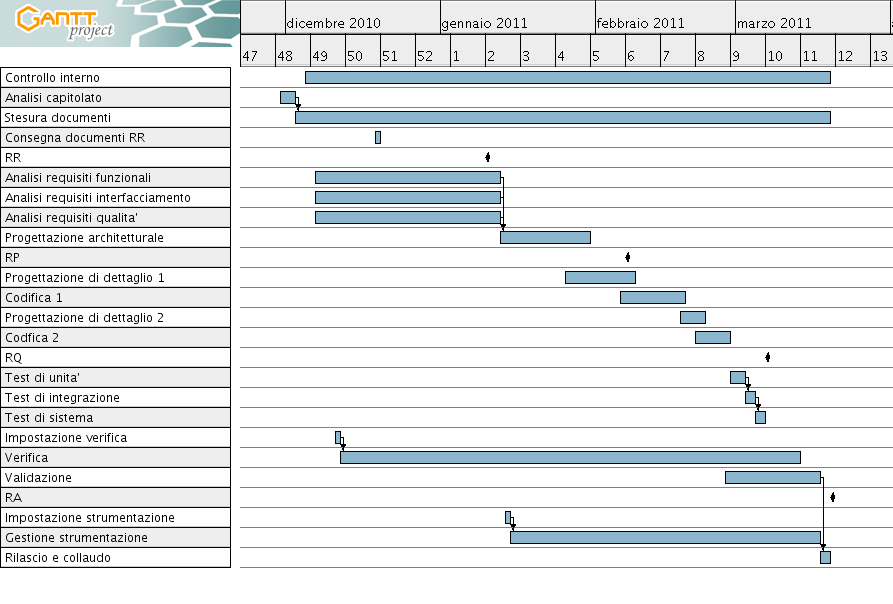
\includegraphics[width=17.2cm, angle=0]{img/PP/gantt1.png}
\caption{Diagramma di Gantt}
\end{figure}
\newpage

Come si pu\`o notare dal grafico, le revisioni sono indicate come punti di
verifica con dei piccoli rombi neri, per semplificare la visione.\\
Si \`e deciso che la fase di analisi proseguir\`a per qualche giorno anche dopo
la RR, per addattare i nostri requisiti ad eventuali variazioni emerse durante
tale revisione.\\

Si pu/`o notare inoltre che la fase di verifica sar/`a presente costantemente a
partire dalla stesura dei documenti, per poi passare alla progettazione e alla
programmazione fino ad arrivare ai test.\\

La stesura dei documenti ricoprir\`a tutta la durata del progetto, poich\`e
verranno aggiornati i documenti stesi nella fase di analisi (Analisi dei
requisiti, Piano di progetto, Piano di Qualifica, Glossario) e verranno stilati
Specifica Tecnica (per la RPP), Definizione di Prodotto (per la RPD interna) e
Manuale Utente (per la RQ).

\section{Prospetto  Economico}
Come specificato nelle richieste del progetto didattico, ciascun ruolo avr\`a un
determinato costo orario (vedi tabella sottostante) che contribuir\`a al calcolo
del costo complessivo del prodotto, che ricordiamo non dovr\`a essere
inferiore a 13.000 Euro.

\vspace{1cm}
\begin{table}[h]
\begin{center}
\begin{tabular}{|l|c|}
\hline
\bo{Ruolo} \cellcolor[gray]{0.9} & \bo{Costo(\euro)}  \cellcolor[gray]{0.9} \\
\hline Responsabile & 30 \\ \hline
Amministratore & 20 \\ \hline
Analista & 25 \\ \hline
Progettista & 22 \\ \hline
Programmatore & 15 \\ \hline
Verificatore & 15 \\
\hline
\end{tabular}
\caption{Ruoli e costi orari}
\end{center}
\end{table}


\vspace{0.5cm}
A partire dalla consegna dei documenti per la RR, verranno tracciate le ore di
lavoro dei membri del gruppo. L'impegno totale di ciascun componente dovr\`a
essere compreso tra 85 e 105 ore, dal quale risulteranno proporzionali
ripartizioni tra carico di lavoro e responsabilit�.\\

Di seguito riportiamo una stima dei costi per ogni revisione e il carico di
lavoro previsto per ogni membro del gruppo.
\newpage

\subsection{RR - RPP}

\vspace{0.5cm}
\bo{Responsabile:} Daminato Simone\\

\bo{Amministratore:} Baron Federico

\vspace{1cm}
\begin{table}[h]
\begin{center}
\begin{tabular}{|l|c|c|c|c|c|c|c|}
\hline
& \bo{Resp.}\cellcolor[gray]{0.9} & \bo{Amm.}\cellcolor[gray]{0.9} &
\bo{Anl.}\cellcolor[gray]{0.9} & \bo{Proget.}\cellcolor[gray]{0.9} &
\bo{Program.}\cellcolor[gray]{0.9} & \bo{Verif.}\cellcolor[gray]{0.9} & \bo{Ore
Totali}\cellcolor[gray]{0.9} \\ \hline

\bo{Baron}\cellcolor[gray]{0.9}    &   & 15 &  5 &  6 & &   & 26 \\ \hline
\bo{Caputo}\cellcolor[gray]{0.9}   &   &    &  5 & 12 & & 5 & 22 \\ \hline
\bo{Daminato}\cellcolor[gray]{0.9} & 12&    &    &  7 & & 6 & 25 \\ \hline
\bo{Lovato}\cellcolor[gray]{0.9}   &   &    & 10 & 10 & &   & 20 \\ \hline
\bo{Mandolo}\cellcolor[gray]{0.9}  &   &    &  8 & 12 & &   & 20 \\ \hline
\bo{Palazzin}\cellcolor[gray]{0.9} &   &    &  6 &  9 & & 5 & 20 \\ \hline
\bo{Trezzi}\cellcolor[gray]{0.9}   &   &    &  7 & 10 & & 6 & 23 \\  \hline

\end{tabular}
\caption{Pianificazione oraria RR-RPP}
\end{center}
\end{table}
\vspace{0.5cm}

\bo{Ore totali:} 156.\\

\bo{Costo previsto per il periodo RR-RPP:} \euro\ 3467.

\vspace{0.8cm}
\begin{figure}[htbp]
  \centering
  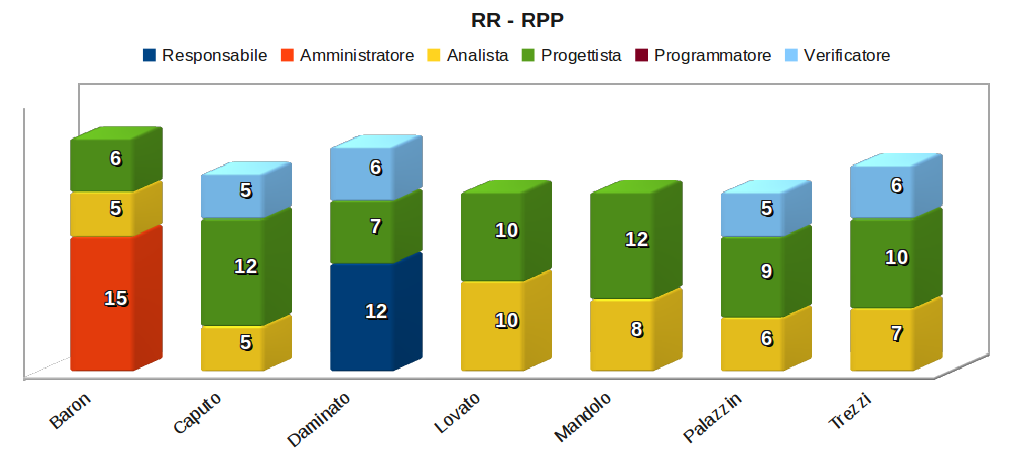
\includegraphics[width=17.2cm, angle=0]{img/PP/RR-RPP.png}
\caption{Distribuzione ore RR-RPP}
\end{figure}
\newpage


\subsection{RPP - RPD}

\vspace{0.5cm}
\bo{Responsabile:} Palazzin Alberto\\

\bo{Amministratore:} Trezzi Giovanni

\vspace{1cm}
\begin{table}[h]
\begin{center}
\begin{tabular}{|l|c|c|c|c|c|c|c|}
\hline
& \bo{Resp.}\cellcolor[gray]{0.9} & \bo{Amm.}\cellcolor[gray]{0.9} &
\bo{Anl.}\cellcolor[gray]{0.9} & \bo{Proget.}\cellcolor[gray]{0.9} &
\bo{Program.}\cellcolor[gray]{0.9} & \bo{Verif.}\cellcolor[gray]{0.9} & \bo{Ore
Totali}\cellcolor[gray]{0.9} \\ \hline

\bo{Baron}\cellcolor[gray]{0.9}    &    &    & 2 & 10 & 7 & 5 & 24 \\ \hline
\bo{Caputo}\cellcolor[gray]{0.9}   &    &    & 4 & 11 &   & 8 & 23 \\ \hline
\bo{Daminato}\cellcolor[gray]{0.9} &    &    & 7 & 12 &   & 5 & 24 \\ \hline
\bo{Lovato}\cellcolor[gray]{0.9}   &    &    &   & 12 & 3 & 7 & 22 \\ \hline
\bo{Mandolo}\cellcolor[gray]{0.9}  &    &    & 2 &  7 & 8 & 7 & 24 \\ \hline
\bo{Palazzin}\cellcolor[gray]{0.9} & 12 &    & 4 & 10 &   &   & 26\\ \hline
\bo{Trezzi}\cellcolor[gray]{0.9}   &    & 13 &   &  9 & 2 &   & 24 \\  \hline

\end{tabular}
\caption{Pianificazione oraria RPP-RPD}
\end{center}
\end{table}
\vspace{0.5cm}

\bo{Ore totali:} 167.\\

\bo{Costo previsto per il periodo RPP-RPD:} \euro\ 3437.

\vspace{0.8cm}
\begin{figure}[htbp]
  \centering
  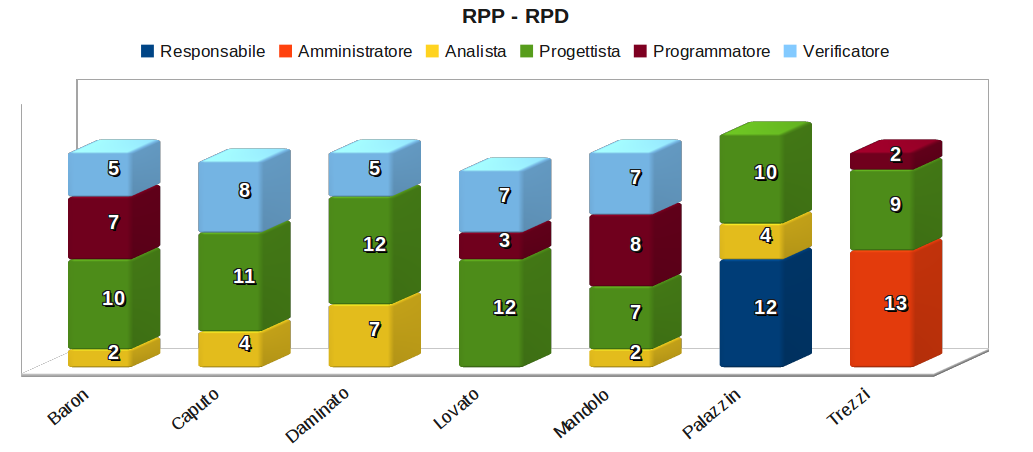
\includegraphics[width=17.2cm, angle=0]{img/PP/RPP-RPD.png}
\caption{Distribuzione ore RPP-RPD}
\end{figure}
\newpage



\subsection{RPD - RQ}

\vspace{0.5cm}
\bo{Responsabile:} Trezzi Giovanni\\

\bo{Amministratore:} Caputo Cosimo

\vspace{1cm}
\begin{table}[h]
\begin{center}
\begin{tabular}{|l|c|c|c|c|c|c|c|}
\hline
& \bo{Resp.}\cellcolor[gray]{0.9} & \bo{Amm.}\cellcolor[gray]{0.9} &
\bo{Anl.}\cellcolor[gray]{0.9} & \bo{Proget.}\cellcolor[gray]{0.9} &
\bo{Program.}\cellcolor[gray]{0.9} & \bo{Verif.}\cellcolor[gray]{0.9} & \bo{Ore
Totali}\cellcolor[gray]{0.9} \\ \hline

\bo{Baron}\cellcolor[gray]{0.9}    &    &    &    &  8 & 15 &  5 & 28 \\ \hline
\bo{Caputo}\cellcolor[gray]{0.9}   &    & 14 &    &    & 16 &  3 & 33 \\ \hline
\bo{Daminato}\cellcolor[gray]{0.9} &    &    &    &  8 & 20 &    & 28 \\ \hline
\bo{Lovato}\cellcolor[gray]{0.9}   &    &    &    &  4 & 21 &  8 & 33 \\ \hline
\bo{Mandolo}\cellcolor[gray]{0.9}  &    &    &    &  8 & 18 &  4 & 30 \\ \hline
\bo{Palazzin}\cellcolor[gray]{0.9} &    &    &    &  4 & 18 &  8 & 30 \\ \hline
\bo{Trezzi}\cellcolor[gray]{0.9}   &  9 &    &    &  3 & 16 &  2 & 30 \\  \hline

\end{tabular}
\caption{Pianificazione oraria RPD-RQ}
\end{center}
\end{table}
\vspace{0.5cm}

\bo{Ore totali:} 212.\\

\bo{Costo previsto per il periodo RPD-RQ:} \euro\ 3630.

\vspace{0.8cm}
\begin{figure}[htbp]
  \centering
  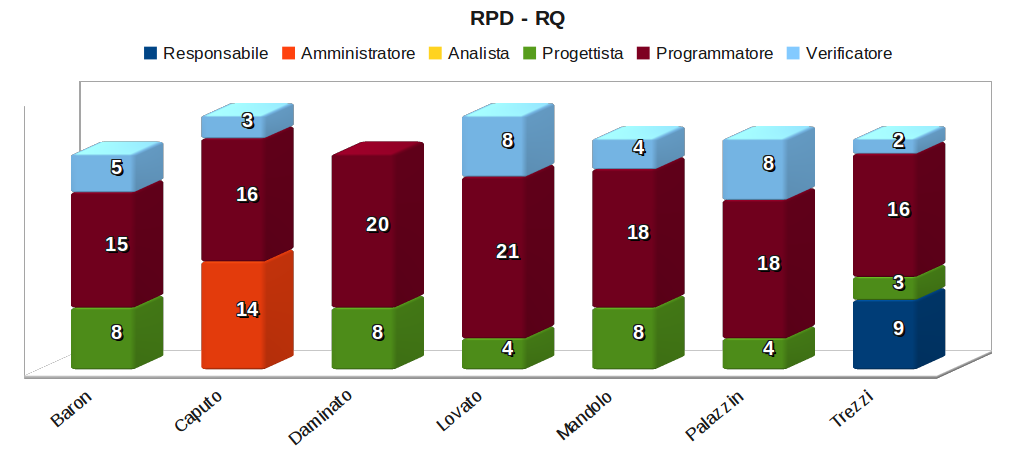
\includegraphics[width=17.2cm, angle=0]{img/PP/RPD-RQ.png}
\caption{Distribuzione ore RPD-RQ}
\end{figure}
\newpage


\subsection{RQ - RA}

\vspace{0.5cm}
\bo{Responsabile:} Mandolo Andrea\\

\bo{Amministratore:} Lovato Daniele

\vspace{1cm}
\begin{table}[h]
\begin{center}
\begin{tabular}{|l|c|c|c|c|c|c|c|}
\hline
& \bo{Resp.}\cellcolor[gray]{0.9} & \bo{Amm.}\cellcolor[gray]{0.9} &
\bo{Anl.}\cellcolor[gray]{0.9} & \bo{Proget.}\cellcolor[gray]{0.9} &
\bo{Program.}\cellcolor[gray]{0.9} & \bo{Verif.}\cellcolor[gray]{0.9} & \bo{Ore
Totali}\cellcolor[gray]{0.9} \\ \hline

\bo{Baron}\cellcolor[gray]{0.9}    &    &    &    &    &  3 & 18 & 21 \\ \hline
\bo{Caputo}\cellcolor[gray]{0.9}   &    &    &    &    &  6 & 15 & 21 \\ \hline
\bo{Daminato}\cellcolor[gray]{0.9} &    &    &    &    &  4 & 18 & 22 \\ \hline
\bo{Lovato}\cellcolor[gray]{0.9}   &    & 13 &    &    &    & 11 & 24 \\ \hline
\bo{Mandolo}\cellcolor[gray]{0.9}  & 10 &    &    &    &    & 15 & 25 \\ \hline
\bo{Palazzin}\cellcolor[gray]{0.9} &    &    &    &    &  7 & 16 & 23 \\ \hline
\bo{Trezzi}\cellcolor[gray]{0.9}   &    &    &    &    &  4 & 18 & 22 \\  \hline

\end{tabular}
\caption{Pianificazione oraria RQ-RA}
\end{center}
\end{table}
\vspace{0.5cm}

\bo{Ore totali:} 158.\\

\bo{Costo previsto per il periodo RQ-RA:} \euro\ 2585.

\vspace{0.8cm}
\begin{figure}[htbp]
  \centering
  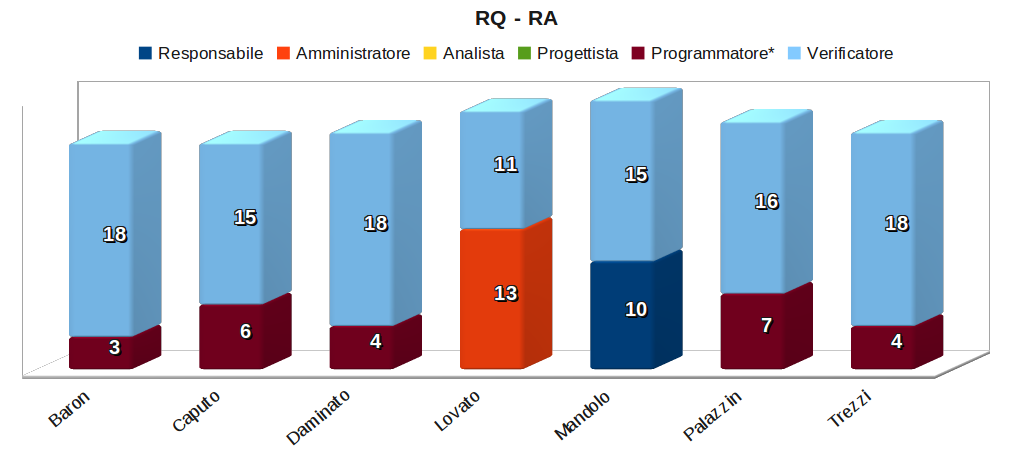
\includegraphics[width=17.2cm, angle=0]{img/PP/RQ-RA.png}
\caption{Distribuzione ore RQ-RA}
\end{figure}
\newpage


\section{Costi complessivi}

\vspace{0.5cm}
In tutto il periodo di sviluppo del software, verranno complessivamente usate
693 ore per un costo totale di \euro\ 13.119,00.

\vspace{1cm}
\begin{table}[h]
\begin{center}
\begin{tabular}{|l|c|c|c|c|c|c|c|}
\hline
& \bo{Resp.}\cellcolor[gray]{0.9} & \bo{Amm.}\cellcolor[gray]{0.9} &
\bo{Anl.}\cellcolor[gray]{0.9} & \bo{Proget.}\cellcolor[gray]{0.9} &
\bo{Program.}\cellcolor[gray]{0.9} & \bo{Verif.}\cellcolor[gray]{0.9} & \bo{Ore
Totali}\cellcolor[gray]{0.9} \\ \hline

\bo{Baron}\cellcolor[gray]{0.9}    &  0 & 15 &  7 & 24 & 25 & 28 & 99 \\ \hline
\bo{Caputo}\cellcolor[gray]{0.9}   &  0 & 14 &  9 & 23 & 22 & 31 & 99 \\ \hline
\bo{Daminato}\cellcolor[gray]{0.9} & 12 &  0 &  7 & 27 & 24 & 29 & 99 \\ \hline
\bo{Lovato}\cellcolor[gray]{0.9}   &  0 & 13 & 10 & 26 & 24 & 26 & 99 \\ \hline
\bo{Mandolo}\cellcolor[gray]{0.9}  & 10 &  0 & 10 & 27 & 26 & 26 & 99 \\ \hline
\bo{Palazzin}\cellcolor[gray]{0.9} & 12 &  0 & 10 & 23 & 25 & 29 & 99 \\ \hline
\bo{Trezzi}\cellcolor[gray]{0.9}   &  9 & 13 &  7 & 22 & 22 & 26 & 99 \\ 
\hline

\end{tabular}
\caption{Pianificazione oraria totale}
\end{center}
\end{table}
\vspace{0.5cm}

Riportiamo qui di seguito un grafico che illustra la ripartizione dei ruoli
sul conto di ore totale.\\



\vspace{0.8cm}
\begin{figure}[htbp]
  \centering
  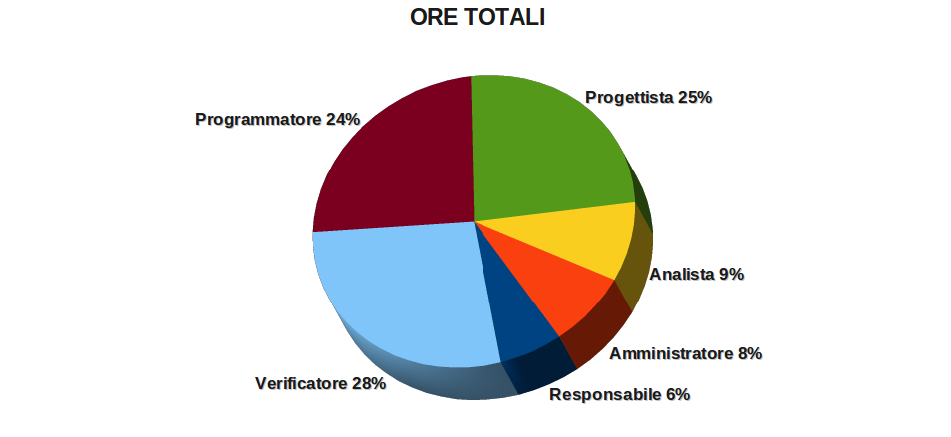
\includegraphics[width=17.2cm, angle=0]{img/PP/totale.png}
\caption{Grafico ripartizione ruoli su ore totali}
\end{figure}


\chapter{Analisi e gestione dei rischi}
\thispagestyle{fancy}

Questo capitolo ha lo scopo di classificare eventuali problematiche per grado
di pericolosit\`a, di analizzarle e di determinare le azioni da intraprendere per
ridurne i danni. L'attenzione ai rischi sar\`a continua nel corso del
progetto.\\ 
Nonostante il nostro gruppo non abbia ancora una visione completa e dettagliata del 
progetto, i rischi che abbiamo individuato sono riportati nelle seguenti sezioni.

\section{Indisposizione dei membri del gruppo}
Grado di pericolosit\`a: alto\\
Per i componenti del VT.G questo progetto \`e una delle prime esperienze nel campo della progettazione software in dettaglio. 
La disponibilit\`a dei membri \`e perci� uno dei rischi maggiori. 
Assenze causate da problematiche fisiche (malattie, incidenti e imprevisti vari) comporterebbero gravi perdite 
di tempo per tutti gli altri membri e conseguenti ritardi nell'avanzamento del
lavoro.\\
\\
Ogni componente \`e tenuto a confermare in modo tempestivo la propria presenza prima di ogni nuovo incontro.
I componenti di VT.G risiedono in differenti zone della regione, i ritrovi devono quindi essere organizzati 
per tempo e comunicati a tutti tempestivamente. Ritardi e/o assenza causa trasporti sono difficilmente gestibili, ma \`e possibile svolgere delle conferenze da casa tramite skype.

\section{Conoscenza delle Tecnologie Utilizzate}
Grado di pericolosit\`a: medio\\
Per la maggior parte dei membri del gruppo questo progetto \`e il primo approccio con tecnologie come Google App Engine, 
perci� almeno inizialmente questo sistema potrebbe risultare problematico e
creare ritardi nello sviluppo.\\
\\ 
\`E stato concordato che ogni membro potr\`a seguire un corso proposto
  dall'azienda di un altro capitolato, quindi le basi per l'utilizzo di questo sistema saranno assicurate per tutti. Il fattore di rischio perci� \`e dettato principalmente dalla difficolt\`a del sistema in s\`e.
Il linguaggio di programmazione adottato (java) non viene considerato come un rischio notevole, in quanto studiato durante il corso di laurea in modo esauriente. 
L'unico inconveniente pu� essere la scrittura del codice del database che sar\`a implentato in GQL, linguaggio simile a SQL 
(ampiamente trattato nel nostro corso di studio).

\section{Usabilit\`a del Prodotto}
Grado di pericolosit\`a: basso\\
Il sistema Netmus \`e un buon prodotto di catalogazione e visualizzazione delle proprie preferenze musicali, 
ma spesso i lettori mp3 che di per s\`e sono gi\`a dispositivi ad alta portabilit\`a mettono a disposizione la visualizzazione del catalogo multimediale, 
aggiornato e ordinato. Inoltre sono presenti altri software simili a
NetMus distribuiti sul web come ad esempio LastFM, molto famoso e
utilizzato nella rete. Ci� potrebbe ridurre
il numero di utenti disposti ad utilizzare il sistema NetMus.\\ 
\\
Una possibile soluzione \`e quella di decorare il progetto con delle
innovative funzionalit\`a, cos� da riuscire ad attirare un maggior numero di clienti.

\section{Strumenti d'Utilizzo}
Grado di pericolosit\`a: medio\\
Altro fattore di rischio identificato \`e l'utilizzo delle strumentazioni adatte. 
Tutti i membri devono utilizzare le stesse strumentazioni e avere le stesse possibilit\`a nel lavoro. 
Guasti hardware, imossibilit\`a di connettersi alla rete Internet, mancanza di strumentazioni software 
adatte comportano ritardi, incompatibilit\`a e sopratutto confusione. \\
\\
Per questo ogni membro del gruppo, 
rispettando le norme di progetto si \`e procurato la strumentazione software adatta prima dell'inizio del 
lavoro, e in caso di problemi pi� complessi \`e invitato a comunicare il fatto al responsabile che cercher\`a una soluzione idonea.

\section{Informazioni Aggiuntive sui Brani Musicali}
Grado di pericolosit\`a: medio\\
I file mp3 da cui si reperiscono i brani spesso non possiedono informazioni
complete, anzi una buona parte di questi file non contiene affatto informazioni, perci� la libreria virtuale 
di un utente risulterebbe composta da molti brani senza titolo,autore e altre
informazioni essenziali.\\ 
\\
Per rendere la liberia virtuale completa di tutte le informazioni si \`e ben pensato di implementare una 
funzione di ricerca automatica nel server dai record di tutti i brani registrati, cos� da completare 
quelli incompleti. Nei casi estremi inoltre sar\`a resa possibile una funzione di inserimento delle informazioni manualmente.

% \chapter{Consuntivo}            da RR in poi
% \thispagestyle{fancy}

\end{document}
